\documentclass[a4paper]{article}

\def\npart {IB}
\def\nterm {Michaelmas}
\def\nyear {2015}
\def\nlecturer {G. R. Grimmett}
\def\ncourse {Markov Chains}
\def\nlectures {TT.10}
\def\nnotready {}

% Imports
\ifx \nextra \undefined
  \usepackage[pdftex,
    hidelinks,
    pdfauthor={Dexter Chua},
    pdfsubject={Cambridge Maths Notes: Part \npart\ - \ncourse},
    pdftitle={Part \npart\ - \ncourse},
  pdfkeywords={Cambridge Mathematics Maths Math \npart\ \nterm\ \nyear\ \ncourse}]{hyperref}
  \title{Part \npart\ - \ncourse}
\else
  \usepackage[pdftex,
    hidelinks,
    pdfauthor={Dexter Chua},
    pdfsubject={Cambridge Maths Notes: Part \npart\ - \ncourse\ (\nextra)},
    pdftitle={Part \npart\ - \ncourse\ (\nextra)},
  pdfkeywords={Cambridge Mathematics Maths Math \npart\ \nterm\ \nyear\ \ncourse\ \nextra}]{hyperref}

  \title{Part \npart\ - \ncourse \\ {\Large \nextra}}
\fi

\author{Lectured by \nlecturer \\\small Notes taken by Dexter Chua}
\date{\nterm\ \nyear}

\usepackage{alltt}
\usepackage{amsfonts}
\usepackage{amsmath}
\usepackage{amssymb}
\usepackage{amsthm}
\usepackage{booktabs}
\usepackage{caption}
\usepackage{enumitem}
\usepackage{fancyhdr}
\usepackage{graphicx}
\usepackage{mathtools}
\usepackage{microtype}
\usepackage{multirow}
\usepackage{pdflscape}
\usepackage{pgfplots}
\usepackage{siunitx}
\usepackage{tabularx}
\usepackage{tikz}
\usepackage{tkz-euclide}
\usepackage[normalem]{ulem}
\usepackage[all]{xy}

\pgfplotsset{compat=1.12}

\pagestyle{fancyplain}
\lhead{\emph{\nouppercase{\leftmark}}}
\ifx \nextra \undefined
  \rhead{
    \ifnum\thepage=1
    \else
      \npart\ \ncourse
    \fi}
\else
  \rhead{
    \ifnum\thepage=1
    \else
      \npart\ \ncourse\ (\nextra)
    \fi}
\fi
\usetikzlibrary{arrows}
\usetikzlibrary{decorations.markings}
\usetikzlibrary{decorations.pathmorphing}
\usetikzlibrary{positioning}
\usetikzlibrary{fadings}
\usetikzlibrary{intersections}
\usetikzlibrary{cd}

\newcommand*{\Cdot}{\raisebox{-0.25ex}{\scalebox{1.5}{$\cdot$}}}
\newcommand {\pd}[2][ ]{
  \ifx #1 { }
    \frac{\partial}{\partial #2}
  \else
    \frac{\partial^{#1}}{\partial #2^{#1}}
  \fi
}

% Theorems
\theoremstyle{definition}
\newtheorem*{aim}{Aim}
\newtheorem*{axiom}{Axiom}
\newtheorem*{claim}{Claim}
\newtheorem*{cor}{Corollary}
\newtheorem*{defi}{Definition}
\newtheorem*{eg}{Example}
\newtheorem*{fact}{Fact}
\newtheorem*{law}{Law}
\newtheorem*{lemma}{Lemma}
\newtheorem*{notation}{Notation}
\newtheorem*{prop}{Proposition}
\newtheorem*{thm}{Theorem}

\renewcommand{\labelitemi}{--}
\renewcommand{\labelitemii}{$\circ$}
\renewcommand{\labelenumi}{(\roman{*})}

\let\stdsection\section
\renewcommand\section{\newpage\stdsection}

% Strike through
\def\st{\bgroup \ULdepth=-.55ex \ULset}

% Maths symbols
\newcommand{\bra}{\langle}
\newcommand{\ket}{\rangle}

\newcommand{\N}{\mathbb{N}}
\newcommand{\Z}{\mathbb{Z}}
\newcommand{\Q}{\mathbb{Q}}
\renewcommand{\H}{\mathbb{H}}
\newcommand{\R}{\mathbb{R}}
\newcommand{\C}{\mathbb{C}}
\newcommand{\Prob}{\mathbb{P}}
\renewcommand{\P}{\mathbb{P}}
\newcommand{\E}{\mathbb{E}}
\newcommand{\F}{\mathbb{F}}
\newcommand{\cU}{\mathcal{U}}
\newcommand{\RP}{\mathbb{RP}}
\newcommand{\CP}{\mathbb{CP}}

\newcommand{\ph}{\,\cdot\,}

\DeclareMathOperator{\sech}{sech}
\DeclareMathOperator{\cosech}{cosech}
\DeclareMathOperator{\cosec}{cosec}

\DeclareMathOperator{\covol}{covol}
\DeclareMathOperator{\vol}{vol}

\let\Im\relax
\let\Re\relax
\DeclareMathOperator{\Im}{Im}
\DeclareMathOperator{\Re}{Re}
\DeclareMathOperator{\im}{im}
\DeclareMathOperator{\image}{image}
\DeclareMathOperator{\Ann}{Ann}

\DeclareMathOperator*{\res}{res}
\DeclareMathOperator{\Res}{Res}
\DeclareMathOperator{\Ind}{Ind}

\DeclareMathOperator{\tr}{tr}
\DeclareMathOperator{\diag}{diag}
\DeclareMathOperator{\rank}{rank}
\DeclareMathOperator{\card}{card}
\DeclareMathOperator{\spn}{span}
\DeclareMathOperator{\adj}{adj}

\DeclareMathOperator{\erf}{erf}
\DeclareMathOperator{\erfc}{erfc}

\DeclareMathOperator{\ord}{ord}
\DeclareMathOperator{\Sym}{Sym}

\DeclareMathOperator{\sgn}{sgn}
\DeclareMathOperator{\orb}{orb}
\DeclareMathOperator{\stab}{stab}
\DeclareMathOperator{\ccl}{ccl}

\DeclareMathOperator{\lcm}{lcm}
\DeclareMathOperator{\hcf}{hcf}

\DeclareMathOperator{\Int}{Int}
\DeclareMathOperator{\id}{id}

\DeclareMathOperator{\betaD}{beta}
\DeclareMathOperator{\gammaD}{gamma}
\DeclareMathOperator{\Poisson}{Poisson}
\DeclareMathOperator{\binomial}{binomial}
\DeclareMathOperator{\multinomial}{multinomial}
\DeclareMathOperator{\Bernoulli}{Bernoulli}
\DeclareMathOperator{\like}{like}

\DeclareMathOperator{\var}{var}
\DeclareMathOperator{\cov}{cov}
\DeclareMathOperator{\bias}{bias}
\DeclareMathOperator{\mse}{mse}
\DeclareMathOperator{\corr}{corr}

\DeclareMathOperator{\otp}{otp}
\DeclareMathOperator{\dom}{dom}

\DeclareMathOperator{\Root}{Root}
\DeclareMathOperator{\supp}{supp}
\DeclareMathOperator{\rel}{rel}
\DeclareMathOperator{\Hom}{Hom}
\DeclareMathOperator{\Aut}{Aut}
\DeclareMathOperator{\Gal}{Gal}
\DeclareMathOperator{\Mat}{Mat}
\DeclareMathOperator{\End}{End}
\DeclareMathOperator{\Char}{char}
\DeclareMathOperator{\ev}{ev}
\DeclareMathOperator{\St}{St}
\DeclareMathOperator{\Lk}{Lk}
\DeclareMathOperator{\disc}{disc}
\DeclareMathOperator{\Isom}{Isom}
\DeclareMathOperator{\length}{length}
\DeclareMathOperator{\energy}{energy}
\DeclareMathOperator{\area}{area}
\DeclareMathOperator{\Syl}{Syl}
\DeclareMathOperator{\cl}{cl}
\DeclareMathOperator{\fix}{fix}

\newcommand{\GL}{\mathrm{GL}}
\newcommand{\SL}{\mathrm{SL}}
\newcommand{\PGL}{\mathrm{PGL}}
\newcommand{\PSL}{\mathrm{PSL}}
\newcommand{\PSU}{\mathrm{PSU}}
\newcommand{\Or}{\mathrm{O}}
\newcommand{\SO}{\mathrm{SO}}
\newcommand{\U}{\mathrm{U}}
\newcommand{\SU}{\mathrm{SU}}

\renewcommand{\d}{\mathrm{d}}
\newcommand{\D}{\mathrm{D}}

\tikzset{->/.style = {decoration={markings,
                                  mark=at position 1 with {\arrow[scale=2]{latex'}}},
                      postaction={decorate}}}
\tikzset{<-/.style = {decoration={markings,
                                  mark=at position 0 with {\arrowreversed[scale=2]{latex'}}},
                      postaction={decorate}}}
\tikzset{<->/.style = {decoration={markings,
                                   mark=at position 0 with {\arrowreversed[scale=2]{latex'}},
                                   mark=at position 1 with {\arrow[scale=2]{latex'}}},
                       postaction={decorate}}}
\tikzset{->-/.style = {decoration={markings,
                                   mark=at position #1 with {\arrow[scale=2]{latex'}}},
                       postaction={decorate}}}
\tikzset{-<-/.style = {decoration={markings,
                                   mark=at position #1 with {\arrowreversed[scale=2]{latex'}}},
                       postaction={decorate}}}

\tikzset{circ/.style = {fill, circle, inner sep = 0, minimum size = 3}}
\tikzset{mstate/.style={circle, draw, blue, text=black, minimum width=0.7cm}}

\definecolor{mblue}{rgb}{0.2, 0.3, 0.8}
\definecolor{morange}{rgb}{1, 0.5, 0}
\definecolor{mgreen}{rgb}{0.1, 0.4, 0.2}
\definecolor{mred}{rgb}{0.5, 0, 0}

\def\drawcirculararc(#1,#2)(#3,#4)(#5,#6){%
    \pgfmathsetmacro\cA{(#1*#1+#2*#2-#3*#3-#4*#4)/2}%
    \pgfmathsetmacro\cB{(#1*#1+#2*#2-#5*#5-#6*#6)/2}%
    \pgfmathsetmacro\cy{(\cB*(#1-#3)-\cA*(#1-#5))/%
                        ((#2-#6)*(#1-#3)-(#2-#4)*(#1-#5))}%
    \pgfmathsetmacro\cx{(\cA-\cy*(#2-#4))/(#1-#3)}%
    \pgfmathsetmacro\cr{sqrt((#1-\cx)*(#1-\cx)+(#2-\cy)*(#2-\cy))}%
    \pgfmathsetmacro\cA{atan2(#2-\cy,#1-\cx)}%
    \pgfmathsetmacro\cB{atan2(#6-\cy,#5-\cx)}%
    \pgfmathparse{\cB<\cA}%
    \ifnum\pgfmathresult=1
        \pgfmathsetmacro\cB{\cB+360}%
    \fi
    \draw (#1,#2) arc (\cA:\cB:\cr);%
}
\newcommand\getCoord[3]{\newdimen{#1}\newdimen{#2}\pgfextractx{#1}{\pgfpointanchor{#3}{center}}\pgfextracty{#2}{\pgfpointanchor{#3}{center}}}

\def\Xint#1{\mathchoice
   {\XXint\displaystyle\textstyle{#1}}%
   {\XXint\textstyle\scriptstyle{#1}}%
   {\XXint\scriptstyle\scriptscriptstyle{#1}}%
   {\XXint\scriptscriptstyle\scriptscriptstyle{#1}}%
   \!\int}
\def\XXint#1#2#3{{\setbox0=\hbox{$#1{#2#3}{\int}$}
     \vcenter{\hbox{$#2#3$}}\kern-.5\wd0}}
\def\ddashint{\Xint=}
\def\dashint{\Xint-}


\begin{document}
\maketitle
{\small
\noindent\textbf{Discrete-time chains}\\
Definition and basic properties, the transition matrix. Calculation of $n$-step transition probabilities. Communicating classes, closed classes, absorption, irreducibility. Calculation of hitting probabilities and mean hitting times; survival probability for birth and death chains. Stopping times and statement of the strong Markov property.\hspace*{\fill} [5]

\vspace{5pt}
\noindent Recurrence and transience; equivalence of transience and summability of $n$-step transition probabilities; equivalence of recurrence and certainty of return. Recurrence as a class property, relation with closed classes. Simple random walks in dimensions one, two and three.\hspace*{\fill} [3]

\vspace{5pt}
\noindent Invariant distributions, statement of existence and uniqueness up to constant multiples. Mean return time, positive recurrence; equivalence of positive recurrence and the existence of an invariant distribution. Convergence to equilibrium for irreducible, positive recurrent, aperiodic chains *and proof by coupling*. Long-run proportion of time spent in a given state.\hspace*{\fill} [3]

\vspace{5pt}
\noindent Time reversal, detailed balance, reversibility, random walk on a graph.\hspace*{\fill} [1]}

\tableofcontents
\setcounter{section}{-1}
\section{Introduction}
So far, in IA Probability, we have always dealt with one random variable, or numerous independent variables, and we were able to handle them. However, in real life, things often \emph{are} dependent, and things become much more difficult. There are many ways in which variables can be dependent. Their dependence can be very complicated, or very simple. We don't really know what to do with them.

This is similar to our study of functions. We can develop theories about continuous functions, increasing functions, or differentiable functions, but if we are just given a random function without assuming anything about it, there really isn't much we can do.

Hence, in this course, we are just going to study a particular kind of dependent variables. In fact, in IA Probability, we did encounter some of these. For example, we dealt with random walks, in which the next position depends on the previous position. This gives us some dependent random variables, but they are dependent in a very simple way.

In reality, a random walk is too simple of a model to describe the world. We need something more general, and these are known as \emph{Markov chains}. These are random distributions that satisfy the \emph{Markov assumption}. This assumption, intuitively, says that the future depends only upon the current state, and not how we got to the current state.

\section{The Markov property}
\begin{defi}[Markov chain]
  Let $\mathbf{X} = (X_0, X_1, \cdots)$ be a sequence of random variables taking values in some set $S$, the \emph{state space}. We assume that $S$ is countable (which could be finite). $\mathbf{X}$ has the \emph{Markov property} if
  \[
    \P(X_{n + 1} = i_{n + 1} | X_0 = i_0, \cdots, X_n = i_n) = \P(X_{n + 1} = i_{n + 1} | X_n = i_n)
  \]
  for all $n\geq 0, i_0,\cdots, i_{n + 1}\in S$.

  If $\mathbf{X}$ has the Markov property, we call it a \emph{Markov chain}.

  We say that a Markov chain $\mathbf{X}$ is \emph{homogeneous} if the conditional probabilities $\P(X_{n + 1} = j | X_n = i)$ do not depend on $n$.
\end{defi}
All our chains $\mathbf{X}$ will be Markov and homogeneous unless otherwise specified.

\begin{eg}\leavevmode
  \begin{enumerate}
    \item A random walk is a Markov chain.
    \item The branching process is a Markov chain.
  \end{enumerate}
\end{eg}

In general, to fully specify a (homogeneous) Markov chain, we will need two items:
\begin{enumerate}
  \item The initial distribution $\lambda_i = \P(X_0 = i)$. We can write this as a vector $\lambda = (\lambda_i: i \in S)$.
  \item The transition probabilities $p_{ij} = \P(X_{n + 1} = j | X_n = i)$. We can write this as a matrix $P = (p_{ij})_{i, j\in S}$.
\end{enumerate}

There are some preliminary properties we know about these items. They are what decide whether a pair $(\lambda, P)$ actually specify a Markov chain.
\begin{prop}\leavevmode
  \begin{enumerate}
    \item $\lambda$ is a \emph{distribution}, ie. $\lambda_i \geq 0, \sum_i \lambda_i = 1$.
    \item $P$ is a \emph{stochastic matrix}, ie. $p_{ij} \geq 0$ and $\sum_j p_{ij} = 1$ for all $i$.
  \end{enumerate}
\end{prop}

\begin{proof}\leavevmode
  \begin{enumerate}
    \item Obvious since $\lambda$ is a probability distribution.
    \item $p_{ij} \geq 0$ since $p_{ij}$ is a probability. We also have
      \[
        \sum_j p_{ij} = \sum_j \P(X_{1} = j | X_0 = i) = 1
      \]
      since $\P(X_1 = \cdot | X_0 = i)$ is a probability distribution function.
  \end{enumerate}
\end{proof}
Note that we only require the row sum to be $1$, and the column sum need not be.

We will prove another seemingly obvious fact.
\begin{thm}
  Let $\lambda$ be a distribution (on $S$) and $P$ a stochastic matrix. The sequence $\mathbf{X} = (X_0, X_1, \cdots)$ is a Markov chain with initial distribution $\lambda$ and transition matrix $P$ iff
  \[
    \P(X_0 = i, X_1 = i_1, \cdots, X_n = i_n) = \lambda_{i_0}p_{i_0 i_1}p_{i_1i_2}\cdots p_{i_{n - 1}i_n}\tag{$*$}
  \]
  for all $n, i_0, \cdots, i_n$
\end{thm}
\begin{proof}
  Let $A_k$ be the event $X_k = i_k$. Then we can write $(*)$ as
  \[
    \P(A_0\cap A_1\cap\cdots \cap A_n) = \lambda_{i_0}p_{i_0 i_1}p_{i_1i_2}\cdots p_{i_{n - 1}i_n}. \tag{$*$}
  \]
  We first assume that $\mathbf{X}$ is a Markov chain. We prove $(*)$ by induction on $n$.

  When $n = 0$, $(*)$ says $\P(A_0) = \lambda_{i_0}$. This is true by definition of $\lambda$.

  Assume that it is true for all $n < N$. Then
  \begin{align*}
    \P(A_0 \cap A_1 \cap \cdots \cap A_N) &= \P(A_0,\cdots, A_{N - 1})\P(A_0, \cdots, A_n | A_0, \cdots, A_{N - 1})\\
    &= \lambda_{i_0} p_{i_0 i_1}\cdots p_{i_{N - 2}i_{N - 1}} \P(A_{N} | A_0,\cdots, A_{N - 1})\\
    &= \lambda_{i_0} p_{i_0 i_1}\cdots p_{i_{N - 2}i_{N - 1}} \P(A_{N} | A_{N - 1})\\
    &= \lambda_{i_0}p_{i_0 i_1}p_{i_1i_2}\cdots p_{i_{N - 1}i_N}.
  \end{align*}
  So it is true for $N$ as well. Hence we are done by induction.

  Conversely, suppose that ($*$) holds. Then for $n = 0$, we have $\P(X_0 = i_0) = \lambda_{i_0}$. Otherwise
  \begin{align*}
    \P(X_n = i_n| X_0 = i_0, \cdots, X_{n - 1} = i_{n - 1}) &= \P(A_n | A_0 \cap \cdots\cap A_{n - 1})\\
    &= \frac{\P(A_0\cap \cdots \cap A_n)}{\P(A_0\cap \cdots \cap A_{n - 1}}\\
    &= p_{i_{n - 1}i_n}
  \end{align*}
  which is independent of $i_0, \cdots, i_{n - 2}$. So this is Markov.
\end{proof}

Often, we do not use the Markov property directly. Instead, we use the following:
\begin{thm}[Extended Markov property]
  Let $\mathbf{X}$ be a Markov chain. For $n \geq 0$, any $H$ given in terms of the past $\{X_i: i < n\}$, and any $F$ given in terms of the future $\{X_i: i > n\}$, we have
  \[
    \P(F| X_n = i, H) = \P(F| X_n = i).
  \]
\end{thm}
To prove this, we need to stitch together many instances of the Markov property. Actual proof is omitted.

\section{Transition probability}
Recall that we specify the Markov chain by the \emph{one-step} transition probability,
\[
  p_{ij} = \P(X_{n + 1} = k: X_n = i).
\]
However, we don't always want to take 1 step. We might want to take 2 steps, 3 steps, or, in general, $n$ steps. We define
\begin{defi}[$n$-step transition probability]
  The $n$-step transition probability from $i$ to $j$ is
  \[
    p_{ij}(n) = \P(X_n = j| X_0 = i).
  \]
\end{defi}
How do we compute these probabilities? We can consider the following question: what is $p_{ij}(m + n)$? We can think of this as a two-step process. We first go form $i$ to some unknown point $k$ after $m$ steps, and then travel from $k$ to $j$ after $n$ more steps. To find the probability to get from $i$ to $j$, we consider all possible routes from $i$ to $j$, and sum up all the probability of the paths. We have
\begin{align*}
  p_{ij}(m + n) &= \P(X_{m + n}| X_0 = i)\\
  &= \sum_k \P(X_{m + n} = j| X_m = k, X_0 = i)\P(X_m = k| X_0 = i)\\
  &= \sum_k \P(X_{m + n} = j| X_m = k)\P(X_m = k: X_0 = i)\\
  &= \sum_k p_{ik}(m)p_{kj}(n)
\end{align*}
\begin{thm}[Chapman-Kolmogorov equation]
  \[
    p_{ij}(m + n) = \sum_{k\in S} p_{ik}(m) p_{kj}(n).
  \]
\end{thm}
This formula is suspiciously familiar. It is just matrix multiplication!

\begin{notation}
  Write $P(m) = (p_{ij}(m))_{i, j\in S}$.
\end{notation}
Then we have
\[
  P(m + n) = P(m)P(n)
\]
In particular, we have
\[
  P(n) = P(1)P(n - 1) = \cdots = P(1)^n = P^n.
\]
This allows us to easily compute the $n$-step transition probability by matrix multiplication.

\begin{eg}
  Let $S = \{1, 2\}$, with
  \[
    P =
    \begin{pmatrix}
      1 - \alpha & \alpha\\
      \beta & 1 - \beta
    \end{pmatrix}
  \]
  We assume $0 < \alpha, \beta < 1$. We want to find the $n$-step transition probability.

  We can achieve this via diagonalization. We can write $P$ as
  \[
    P = U^{-1}
    \begin{pmatrix}
      \kappa_1 & 0\\
      0 & \kappa_2
    \end{pmatrix}U,
  \]
  where the $\kappa_i$ are eigenvalues of $P$, and $U$ is composed of the eigenvectors.

  To find the eigenvalues, we calculate
  \[
    \det (P - \lambda I) = (1 - \alpha - \lambda)(1 - \beta - \lambda) - \alpha\beta = 0.
  \]
  We solve this to obtain
  \[
    \kappa_1 = 1,\quad \kappa_2 = 1 - \alpha - \beta.
  \]
  Usually, the next thing to do would be to find the eigenvectors to obtain $U$. However, here we can cheat a bit and not do that. Using the diagonalization of $P$, we have
  \[
    P^n = U^{-1}
    \begin{pmatrix}
      \kappa_1^n & 0\\
      0 & \kappa_2^n
    \end{pmatrix}U.
  \]
  We can now attempt to compute $p_{12}$. We know that it must be of the form
  \[
    p_{12} = A\kappa_1^n + B\kappa_2^n = A + B(1 - \alpha - \beta)^n
  \]
  where $A$ and $B$ are constants coming from $U$ and $U^{-1}$. However, we know well that
  \[
    p_{12}(0) = 0,\quad p_{12}(1) = \alpha.
  \]
  So we obtain
  \begin{align*}
    A + B &= 0\\
    A + B(a - \alpha - \beta) &= \alpha.
  \end{align*}
  This is something we can solve, and obtain
  \[
    p_{12}(n) = \frac{\alpha}{\alpha + \beta}(1 - (1 - \alpha - \beta)^n) = 1 - p_{11}(n).
  \]
  How about $p_{21}$ and $p_{22}$? Well we don't need additional work. We can obtain these simply by interchanging $\alpha$ and $\beta$. So we obtain
  \[
    P^n = \frac{1}{\alpha + \beta}
    \begin{pmatrix}
      \beta + \alpha(1 - \alpha - \beta)^n & \alpha - \alpha(1 - \alpha - \beta)^n\\
      \alpha + \beta(1 - \beta - \alpha)^n & \beta - \beta(1 - \beta - \alpha)^n
    \end{pmatrix}
  \]
  What happens as $n\to \infty$? We can take the limit and obtain
  \[
    P^n \to \frac{1}{\alpha + \beta}
    \begin{pmatrix}
      \beta & \alpha\\
      \beta & \alpha
    \end{pmatrix}
  \]
  We see that the two rows are the same. This means that as time goes on, where we end up does not depend on where we started.

  Alternatively, we can solve this by a difference equation. We have
  \[
    p_{11}(n + 1) = p_{11}(n)(1 - \alpha) + p_{12}(n)\beta = p_{11}(n)(1 - \alpha) + (1 - p_{11}(n))\beta.
  \]
  We can solve this as we have done in IA differential equations.
\end{eg}
As in the Chapman-Kolmogorov equation, many statements about Markov chains can be concisely stated in the language of linear algebra.

In general, let $X_0$ have distribution $\lambda$. What is the distribution of $X_1$? We have
\[
  \P(X_i = j) = \sum_i \P(X_1 = j| X_0 = i)\P(X_0 = i) = \sum_i \lambda_i p_{ij}.
\]
Hence this has a distribution $\lambda P$, where $\lambda$ is treated as a row vector. Similarly, $X^n$ has the distribution $\lambda P^n$.

In fact, historically, Markov chains was initially developed as a branch of linear algebra. However, nowadays, we often look at it as a branch of probability theory instead, and this is what we will do in this course. So don't be scared if you hate linear algebra.

\subsection{Class structure}
\begin{defi}[Leading to and communicate]
  Suppose we have two states $i, j\in S$. We write $i \to j$ ($i$ \emph{leads to} $j$) if there is some $n \geq 0$ such that $p_{ij}(n) > 0$, ie. it is possible for us to get from $i$ to $j$ (in multiple steps). Note that we allow $n = 0$.

  We write $i \leftrightarrow j$ if $i \to j$ and $j \to i$. If $i \leftrightarrow j$, we say $i$ and $j$ ``communicate''
\end{defi}

\begin{prop}
  $\leftrightarrow$ is an equivalence relation.
\end{prop}

\begin{proof}\leavevmode
  \begin{enumerate}
    \item Reflexive: we have $i \leftrightarrow i$ since $p_{ii}(0) = 1$.
    \item Symmetric: trivial by definition.
    \item Transitive: suppose $i \to j$ and $j \to k$. Since $i \to j$, there is some $m > 0$ such that $p_{ij}(m) > 0$. Since $j \to k$, there is some $n$ such that $p_{jk}(n) > 0$. Then $p_{ik}(m + n) = \sum_{r} p_{ir}(m)p_{r k}(n) \geq p_{ij}(m)p_{jk}(n) > 0$. So $i \to k$.

      Similarly, if $j \to i$ and $k \to j$, then $k \to i$. So $i \leftrightarrow j$ and $j \leftrightarrow k$ implies that $i \leftrightarrow k$.
  \end{enumerate}
\end{proof}
So we have an equivalence relation, and we know what to do with equivalence relations. We form equivalence classes!
\begin{defi}[Communicating classes]
  The equivalence classes of $\leftrightarrow$ are \emph{communicating classes}.
\end{defi}
We have to be careful with these communicating classes. They are not completely isolated. Within a communicating class $A$, of course we can move between any two vertices. However, it is possible that we can escape from a class $A$ to a class $B$. It is just that after going to $B$, we cannot go back to class $A$. From $B$, we might be able to get to another space $C$. We can jump around all the time, but (if there are finitely many communicating classes) eventually we have to stop when we have visited every class. Then we are bound to stay in that class.

Since we are eventually going to be stuck in that class anyway, often, we can just consider this final communicating class and ignore the others. So wlog we can assume that the chain only has one communicating class.

\begin{defi}[Irreducible chain]
  A Markov chain is \emph{irreducible} if there is a unique communication class.
\end{defi}

\begin{defi}[Closed]
  A subset $C\subseteq S$ is \emph{closed} if $p_{ij} = 0$ for all $i \in C, j\not\in C$.
\end{defi}

\begin{prop}
  A subset $C$ is closed iff ``$i\in C, i\to j$ implies $j \in C$''.
\end{prop}

\begin{proof}
  Assume $C$ is closed. Let $i \in C, i \to j$. Since $i \to j$, there is some $m$ such that $p_{ij}(m) > 0$. Expanding the Chapman-Kolmogorov equation, we have
  \[
    p_{ij}(m) = \sum_{i_1, \cdots, i_{m - 1}} p_{i, i_1}p_{i_1, i_2}, \cdots, p_{i_{m - 1},j} > 0.
  \]
  So there is some route $i, i_1, \cdots, i_{m - 1}, j$ such that $p_{i, i_1}, p_{i_1, i_2}, \cdots, p_{i_{m - 1}, j} > 0$. Since $p_{i, i_1} > 0$, we have $i_1\in C$. Since $p_{i_1,i_2} > 0$, we have $i_2\in C$. By induction, we get that $j \in C$.

  To prove the other direction, assume that ``$i\in C, i \to j$ implies $j\in C$''. So for any $i\in C, j\not\in C$, then $i\not\to j$. So in particular $p_{ij} = 0$.
\end{proof}

\begin{eg}
  Consider $S = \{1, \cdots, 6\}$ with transition matrix
  \[
    P =
    \begin{pmatrix}
      \frac{1}{2} & \frac{1}{2} & 0 & 0 & 0 & 0\\
      0 & 0 & 1 & 0 & 0 & 0\\
      \frac{1}{3} & 0 & 0 & \frac{1}{3} & \frac{1}{3} & 0\\
      0 & 0 & 0 & \frac{1}{2} & \frac{1}{2} & 0\\
      0 & 0 & 0 & 0 & 0 & 1\\
      0 & 0 & 0 & 0 & 1 & 0\\
    \end{pmatrix}
  \]
  \begin{center}
    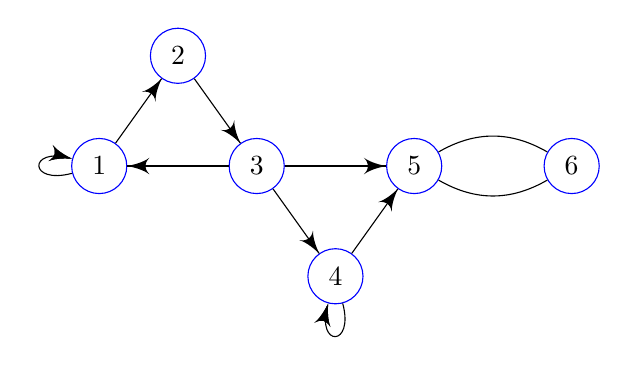
\begin{tikzpicture}
      \node [mstate] (1) at (0, 0) {$1$};
      \node [mstate] (2) at (1, 1.4) {$2$};
      \node [mstate] (3) at (2, 0) {$3$};
      \node [mstate] (4) at (3, -1.4) {$4$};
      \node [mstate] (5) at (4, 0) {$5$};
      \node [mstate] (6) at (6, 0) {$6$};
      \draw (1) edge [loop left, ->] (1);
      \draw (1) edge [->] (2);
      \draw (2) edge [->] (3);
      \draw (3) edge [->] (1);
      \draw (3) edge [->] (4);
      \draw (3) edge [->] (5);
      \draw (4) edge [->] (5);
      \draw (4) edge [loop below, ->] (4);
      \draw (5) edge [bend left, ->] (6);
      \draw (6) edge [bend left, ->] (5);
    \end{tikzpicture}
  \end{center}
  We see that the communicating classes are $\{1, 2, 3\}$, $\{4\}$, $\{5, 6\}$, where $\{5, 6\}$ is closed.
\end{eg}

\section{Recurrence or transience}
We adopt the following notation:
\[
  \P_i(A) = \P(A| X_0 = i),
\]
and
\[
  \E_i(Z) = \E(Z| X_0 = i).
\]
Suppose we start from $i$, and randomly wander around. Eventually, we may or may not get to $j$. If we do, there is a time at which we first reach $j$. We call this the \emph{first passage time}, written
\[
  T_j = \min\{n \geq 1: X_n = j\}.
\]
Note that we require $n \geq 1$. Otherwise $T_i$ would always be $0$.

The \emph{first passage probability} is
\[
  f_{ij}(n) = \P_i(T_j = n).
\]
\begin{defi}[Recurrent state]
  A state $i\in S$ is \emph{recurrent} (or \emph{persistent}) if
  \[
    \P_i (T_i < \infty) = 1,
  \]
  ie. we will eventually get back to the space. Otherwise, we call the state \emph{transient}.
\end{defi}
Note that transient does \emph{not} mean we don't get back. It's just that we are not sure that we will get back. We can (but will not) show that if a state is recurrent, then the probability that we return to $i$ infinitely many times is also $1$.

Note that when we discuss about recurrent and transient states, we are often concerned with an infinite state space. In the infinite state space, a state is transient because we are likely to wander to a place far far away and not get back. However, in a finite state space, transience happens only if we are stuck somewhere, ie. we are not in an irreducible state space. This is not too interesting.

Our current objective is to show the following:
\begin{thm}
  $i$ is recurrent iff $\sum_n p_{ii}(n) = \infty$.
\end{thm}
The technique to prove this would be to use generating functions. We need to first decide what sequence to work with. For any fixed $i, j$, consider the sequence $p_{ij}(n)$ as a sequence in $n$. Then we define
\[
  P_{ij}(s) = \sum_{n = 0}^\infty p_{ij}(n) s^n.
\]
We also define
\[
  F_{ij}(S) = \sum_{n = 0}^\infty f_{ij}(n) s^n,
\]
where $f_{ij}$ is our first-pass probability. For the sake of clarity, we make it explicit that $p_{ij}(0) = \delta_{ij}$, and $f_{ij}(0) = 0$.

Our proof would be heavily based on the result below:
\begin{thm}[]
  \[
    P_{ij}(s) = \delta_{ij} + F_{ij}(s)P_{jj}(s),
  \]
  for $-1 < s \leq 1$.
\end{thm}

\begin{proof}
  Using the law of total probability
  \begin{align*}
    p_{ij}(n) &= \sum_{m = 1}^n \P_i(X_n = j| T_j = m) \P_i(T_j = m) \\
    \intertext{Using the Markov property, we can write this as}
    &= \sum_{m = 1}^n \P(X_n = j| X_m = j) \P_i(T_j = m)\\
    &= \sum_{m = 1}^n p_{jj}(n - m) f_{ij}(m).
  \end{align*}
  We can multiply through by $s^n$ and sum over all $n$ to obtain
  \[
    \sum_{n = 1}^\infty p_{ij}(n) S^n = \sum_{n = 1}^\infty \sum_{m = 1}^n p_{jj}(n - m)s^{n - m} f_{ij}(m)s^m.
  \]
  The left hand side is \emph{almost} the generating function $P_{ij}(s)$, except that we are missing an $n = 0$ term, which is $p_{ij}(0) = \delta_{ij}$. The right hand side is the ``convolution'' of the power series $P_{jj}(s)$ and $F_{ij}(s)$, which we can write as the product $P_{jj}(s) F_{ij}(s)$. So
  \[
    P_{ij}(s) - \delta_{ij} = P_{ij}(s) F_{ij}(s).
  \]
\end{proof}

Before we actually prove our theorem, we need one helpful result from Analysis that allows us to deal with power series nicely.
\begin{lemma}[Abel's lemma]
  Let $u_1, u_2, \cdots$ be real numbers such that $U(s) = \sum_{n} u_n s^n$ converges for $0 < s < 1$. Then
  \[
    \lim_{s\to 1^-} U(s) = \sum_n u_n.
  \]
\end{lemma}
Proof is an exercise for Analysis.

We now prove the theorem we initially wanted to show
\begin{thm}
  $i$ is recurrent iff $\sum_n p_{ii}(n) = \infty$.
\end{thm}

\begin{proof}
  Using $j = i$ in the above formula, for $0 < s < 1$, we have
  \[
    P_{ii}(s) = \frac{1}{1 - F_{ii} (s)}.
  \]
  Here we need to be careful that we are not dividing by $0$. Thiw would be a problem if $F_{ii}(s) = 1$. By definition, we have
  \[
    F_{ii}(s) = \sum_{n = 1}^\infty f_{ii}(n) s^n.
  \]
  Also, by definition of $f_{ii}$, we have
  \[
    F_{ii}(1) = \sum_n f_{ij}(n) = \P(\text{ever returning to }1) \leq 1.
  \]
  So for $|s| < 1$, $F_{ii}(s) < 1$. So we are not dividing by zero. Now we use our original equation
  \[
    P_{ii}(s) = \frac{1}{1 - F_{ii} (s)},
  \]
  and take the limit as $s \to 1$. By Abel's lemma, we know that the left hand side is
  \[
    \lim_{s \to 1}P_{ii}(s) = P_{ii}(1) = \sum_n p_{ii}(n).
  \]
  The other side is
  \[
    \lim_{s \to 1}\frac{1}{1 - F_{ii}(s)} = \frac{1}{1 - \sum f_{ii}(n)}.
  \]
  Hence we have
  \[
    \sum_n p_{ii}(n) = \frac{1}{1 - \sum f_{ii}(n)}.
  \]
  Since $\sum f_{ii}(n)$ is the probability of ever returning, the probability of ever returning is 1 if and only if $\sum_n p_{ii}(n) = \infty$.
\end{proof}

Using this result, we can check if a state is recurrent. However, a Markov chain has many states, and it would be tedious to check if every state is recurring. Thus we have the following helpful result.
\begin{thm}[]
  Let $C$ be a communicating class. Then
  \begin{enumerate}
    \item Either every state in $C$ is recurrent, or every state is transient.
    \item If $C$ contains a recurrent state, then $C$ is closed.
  \end{enumerate}
\end{thm}

\begin{proof}\leavevmode
  \begin{enumerate}
    \item Let $i \leftrightarrow j$ and $i \not =j$. Then by definition of communicating, there is some $m$ such that $p_{ij}(m) = \alpha > 0$, and some $n$ such that $p_{ji}(n) = \beta > 0$. So for each $k$, we have
      \[
        p_{ii}(m + k + n) \geq p_{ij}(m) p_{jj}(k) p_{ji}(n) = \alpha\beta p_{jj}(k).
      \]
      So if $\sum_k p_{jj}(k) = \infty$, then $\sum_r p_{ii}(r) = \infty$. So $j$ recurrent implies $i$ recurrent. Similarly, $i$ recurrent implies $j$ recurrent.
    \item If $C$ is not closed, then there is a non-zero probability that we leave the class and never get back. So the states are not recurrent.
  \end{enumerate}
\end{proof}

Note that there is a profound difference between a finite state space and an infinite state space. A finite state space can be represented by a finite matrix, and we are all very familiar with a finite matrices. We can use everything we know about finite matrices from IA Vectors and Matrices. However, infinite matrices are weirder.

For example, any finite transition matrix $P$ has an eigenvalue of $1$. This is since the row sums of a transition matrix is always $1$. So if we multiply $P$ by $\mathbf{e} = (1, 1, \cdots, 1)$, then we get $\mathbf{e}$ again. However, this is not true for infinite matrices, since we usually don't usually allow arbitrary infinite vectors. We usually restrict our focus to vectors $\mathbf{x}$ such that $\sum x_i^2$ is finite. In this case the vector $\mathbf{e}$ is not allowed, and the transition matrix need not have eigenvalue $1$.

Another thing about a finite state space is that probability ``cannot escape''. We can think of a Markov chain as a flow of probabilities around the state space, with the probability distribution moving around in every step. If we have a finite state space, all the probability must be contained within your finite state space. However, if we have an infinite state space, then probabilities can just drift away to infinity.

In particular, we have the following result:
\begin{thm}[]
  In a finite state space,
  \begin{enumerate}
    \item There exists at least one recurrent state.
    \item If the chain is irreducible, every state is recurrent.
  \end{enumerate}
\end{thm}

\begin{proof}
  Recall that
  \[
    P_{ij}(s) = \delta_{ij} + P_{jj}(s) F_{ij}(s).
  \]
  If $j$ is transient, then $\sum_n p_{jj}(n) = P_{jj}(1) < \infty$. Hence $P_{ij}(1) < \infty$. By Abel's lemma, $P_{ij}(1)$ is given by
  \[
    P_{ij}(1) = \sum_n p_{ij}(n).
  \]
  Since this is finite,  we must have $p_{ij}\to 0$.

  Since we know that
  \[
    \sum_{j\in S}p_{ij}(n) = 1,
  \]
  If every state is transient, then for all $j$, $\sum p_{ij}(n) \to 0$ as $n\to \infty$. This is a contradiction.
\end{proof}

\begin{thm}[P\'olya's theorem]
  Consider $\Z^d = \{(x_1, x_2, \cdots, x_d): x_i \in \Z\}$. This generates a graph with $x\sim y$ if $|x - y| = 1$, where $|\cdot |$ is the Euclidean norm.
  \begin{center}
    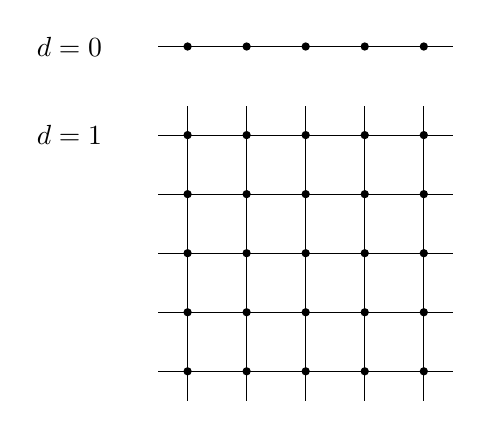
\begin{tikzpicture}[scale=0.75]
      \node at (-4, 0) {$d = 0$};
      \draw (-2.5, 0) -- (2.5, 0);
      \foreach \x in {-2,-1,...,2} {
        \node [circ] at (\x, 0) {};
      }
      \begin{scope}[shift={(0, -3.5)}]
        \node at (-4, 2) {$d = 1$};
        \foreach \x in {-2, -1,...,2} {
          \foreach \y in {-2,-1,...,2} {
            \node [circ] at (\x, \y) {};
          }
        }
        \foreach \x in {-2, -1,...,2} {
          \draw (\x, -2.5) -- (\x, 2.5);
          \draw (-2.5, \x) -- (2.5, \x);
        }
      \end{scope}
    \end{tikzpicture}
  \end{center}
  Consider a random walk in $\Z^d$. At each step, it moves to a neighbour, each chosen with equal probability. Then this is recurrent if $d = 1$ or $2$.
\end{thm}
\end{document}
